\documentclass[main.tex]{subfiles}

\begin{document}

\chapter{Equilibrio idrostatico}
\PartialToc

\section{Vincoli osservativi}
Even for the best observed star we observe just 4 basic items

\begin{itemize*}
\item Mass
\item Luminosity
\item Radius
\item  Composition of outer layer
\end{itemize*}

\subsection{Stars: autogravitating bodies in internal equilibrium.}
These items couldn't suffice to derive uniquely the internal structure if it were not for one additional observed item: the constancy of stars over long time intervals (Alghe fossili: luminosit\'a del sole approx. costante per 1 miliardo di anni. Periodo delle Cefeidi lentamente variabile($\tau\approx$ 1 milione yr)): the stellar interior must be in perfect equilibrium.

\section{Fluidodinamica: equazione di Navier-Stokes}

\subsection{Formulazione Euleriana}
Le propriet\'a del fluido come $P,\,T,\,\rho,\,\vec{v},\,\ldots$ sono campi scalari o vettoriali dipendenti dalle variabili posizion $\vec{r}$ e del tempo t: $\vec{r}$ is the position of observer so its time derivative is meaningless without qualification.

Introduco la derivata di Stokes (materiale)\index{Derivata di Stokes (materiale)}

\begin{align*}
D/Dt=\frac{d}{dt}=\frac{\partial}{\partial t}+\scap{v}{\nabla}&\intertext{dove il gradiente  \'e l'operatore tradizionale e la velocit\'a si riferisce a un elemento di fluido}\\
\vec{v}(\vec{r},t)=\frac{d\vec{r}}{dt}=\dot{\vec{r}}&\intertext{$\vec{r}$ \'e una variabile lagrangiana}
\end{align*}



\subsection{Formulazione Lagrangiana.}

Nella formulazione Lagrangiana seguo il moto di ogni dato elemento di fluido: in this description $\vec{r}$ denotes the position of fluid element and is no more an indipendent variable rather is a function of t and (in 3D) of 3 parameter. If the parameters form a position vector which was identical to position vector at $t=0$ then $\vec{r}=\vec{r}(\vec{a},t)$.

The a's don't need to be coordinates in Lagr. desc.: in 1D (spherical symmetry) a may denotes physical properties of the fluid element at some prior time.

In spherically symmetric case it's convenient to take a Lagrangian coordinate instead of r:
we choose m and any other variables dependes on m and t.

For star of constant mass the radius $R=r(M,t)$ vary strongly in time while $0\leq m\leq M$.


\subsection{Leggi di conservazione}

\subsubsection{Conservation of mass}

\begin{align*}
&\PDy{t}{\rho}+\nabla\cdot(\rho\vec{v})=0&\intu{in Eulerian description mass conservation is expressed as continuity equation, and in term of specific volume $v=\frac{1}{\rho}$:}\\
&\frac{1}{v}\TDy{t}{v}=\scap{\nabla}{v}
\end{align*}

\subsubsection{Momentum conservation}

$v_i$ are components of particles velocities:

\begin{align*}
&\exv{v_iv_k}=u_iu_k+\exv{w_iw_k}\\
&P=\frac{1}{3}\rho\exv{|\vec{w}|^2}=\frac{2}{3}U_{kin}\\
&(\\
&u=\frac{1}{\rho}\intzi{}\TDy{p}{n(p)}\epsilon(p)\,dp,\\ &U_{kin}=\intzi{}\TDy{p}{n(p)}\epsilon(p)\,dp\\
&u=\frac{1}{\rho}\intzi{}n\frac{4\pi p^2}{(2\pi mkT)\expy{\frac{3}{2}}}\exp{-\frac{p^2}{2mkT}}(\frac{p^2}{2m})\,dp=\frac{3}{2}\frac{P}{\rho}\\
&\epsilon(p)=mc^2(\sqrt{1+\frac{p^2}{m^2c^2}}-1)\\
&):\\
&u=\frac{1}{\rho}\intzi{}(\frac{c}{kT})^3\frac{n}{2}p^2\exp{-\frac{pc}{kT}}(pc)\,dp=3\frac{P}{\rho}\\
&U_{rad}=aT^4=3P_{rad})\\
&\rho\exv{w_iw_k}=P\delta_{ik}-\pi_{ik}&\intertext{$\pi_{ik}$ is the viscous stress tensor\index{Viscous stress tensor}:}\\
&\pi_{ik}=\rho\exv{\frac{1}{3}|\vec{w}|^2\delta_{ik}-w_iw_k}\\
&\PDof{t}(\rho u_i)+\PDof{x_k}(\rho u_iu_k+P\delta_{ik}-\pi_{ik})=\rho f_i\\
&\rho\TDy{t}{v_i}=-\PDof{x_j}P\indices{_i_j}+\rho f_i&\intu{in eulerian description: $\vec{v}$ is the momentum per unit mass $P$ total pressure tensor (symmetric in order to conserve angular momentum), assume mass conservation.}\\
&\PDy{t}{(\rho v_i)}+\PDof{x_j}(\rho v_iv_j+P_{ij})=\rho f_i&\intu{conservation form, doesn't require mass conservation}\\
&(\rho v_iv_j+P_{ij})&\intu{Rate of flow of momentum of flux\index{Rate of flow of momentum of flux}}
\end{align*}

\subsubsection{Energy conservation}

\begin{align*}
&\PDof{t}[\frac{\rho}{2}(|\vec{u}|^2+\exv{|\vec{w}|^2})]\\
&+\PDof{x_k}[\frac{\rho}{2}\exv{(u_k+w_k)(u_i+w_i)^2}]-\rho f_ku_k=0\\
&\TDof{t}(\frac{1}{2}\vec{v}^2)=-\frac{1}{\rho}\vec{v}\cdot(\nabla\cdot P)+\scap{f}{v}\\
&\PDof{t}(\frac{\rho}{2}|\vec{u}|^2+\rho U)\\
&+\PDof{x_k}[\frac{\rho}{2}|\vec{u}|^2u_k+u_i(P\delta_{ik}-\pi_{ik})\rho Uu_k+F_k]\\
&=\rho u_kf_k&\intu{states that the total fluid energy density is  the sum of a part due to bulk motion $\rho|\vec{u}|^2$ and a part due to random motion $U \rho$; the flux of fluid in k direction consist of translation of bulk of kinetic energy at k component of mean velocity $\frac{\rho}{2}|\vec{u}|^2u_k$, plus enthalpy flux $(\rho U+P)u_k$, plua viscous contribution $-u_i\pi_{ki}$, plus conductive flux $F_k$}
&\rho U=\rho\exv{\frac{1}{2}|\vec{w}|^2}&\intu{$U$ is the specific internal energy}\\
&F_k=\rho\exv{w_k\frac{1}{2}|\vec{w}|^2}&\intu{conduction heat flux}\\
&\PDof{t}\frac{\rho}{2}|\vec{u}|^2+\PDof{x_k}(\frac{\rho}{2}|\vec{u}|^2u_k)\\
&=\rho u_if_i-u_i\PDy{x_i}{P}+u_i\PDy{x_k}{\pi_{ik}}&\intu{work equation}\\
&\PDof{t}(\rho U)+\PDof{x_k}(\rho Uu_k)=-P\PDy{x_k}{u_k}-\PDy{x_k}{F_k}+\Psi&\intu{internal energy equation}\\
&\Psi=\pi_{ik}\PDy{x_k}{u_i}&\intu{rate of viscous dissipation}\\
&\rho\TDy{t}{U}=-P\scap{\nabla}{u}-\scap{\nabla}{F}_{con}+\Psi\intu{internal energy equation in the form of first law of thermodynamic}\\
&-P\scap{\nabla}{u}=-P[\rho\TDy{t}{(\rho\expy{-1})}]&\intu{rate of doing $P\,dV$ work}\\
&-\scap{\nabla}{F}_{con}+\Psi&\intu{rate of adding heat}
\end{align*}

\subsection{First basic equation in Eulerian description}
For gaseus non-rotating single stars without strong magnetic field the only forces acting on a mass element are pressure and gravity.

Scelgo r e t come variabili indipendenti: $\rho(r,t)$, $m(r,t)$.

\begin{align*}
&dm=4\pi r^2\rho\,dr-4\pi r^2\rho v\,dt&\intertext{the first term is the mass contained in a spherical shell of thickness $dr$ and it gives the variation of $m(r,t)$ due to variation of r at constant t:}\\
&\frac{\partial m}{\partial r}=4\pi r^2\rho&\intertext{$\uparrow$ is our first basic eq in E description.}\\
&\frac{\partial m}{\partial t}=-4\pi r^2\rho v&\intertext{explain the last term in first equation that gives the spherically simmetric mass flow out of sphere of constant radius due to velocity v in outward direction in time $dt$}
\end{align*}

Differenziando opportunamente ottengo l'equazione di continuit\'a
\begin{align*}
&\frac{\partial \rho}{\partial t}=-\frac{1}{r^2}\frac{\partial(\rho r^2 v)}{\partial r}&\intertext{$\uparrow$ \'e la forma per simmetria sferica dell'equazione di C:}\\
&\frac{\partial \rho}{\partial t}=-\nabla\cdot(\rho\vec{v})
\end{align*}

\subsection{Connessione tra E. e L. desc.}

For any function of 2 variables if one is substituted $(r,t\to m,t)$ 

\begin{align*}
\frac{\partial}{\partial m}=\frac{\partial}{\partial r}\frac{\partial r}{\partial m}&\intertext{che applicata ad m:}\\
\frac{\partial r}{\partial m}=\frac{1}{4\pi r^2 \rho}&\intertext{$\uparrow$ is the first basic equation in L. desc.}\\
(\frac{\partial}{\partial t})_m=\frac{\partial}{\partial r}(\frac{\partial r}{\partial t})_m+(\frac{\partial}{\partial t})_r&\intertext{$\uparrow$ substantial derivative of hydrodynamic}
\end{align*}


\subsection{Equazione del moto}

Tensore flusso d'impulso

\begin{equation*}
\Pi_{ik}=P\delta_{ik}+\rho v_iv_k
\end{equation*}

Equazione del moto in desc. L
\begin{align*}
&\rho\frac{d\vec{v}}{dt}=-\nabla\cdot P+\rho \vec{f}\\
&\frac{\partial}{\partial t}(\rho v_i)=-\frac{\partial}{\partial x_k}\Pi_{ik}+\rho f_i&\intertext{$\vec{v}$ is the fluid velocity (linear momentum per unit mass), $\vec{f}$ is the total body or external force per unit mass.}
\end{align*}

\subsection{Equazione di Eulero: lowest order solution}

\subsection{Navier-Stokes equation: first order approximation}

\subsection{Fluido incompressibile: equazione di Navier-Stokes}

Per un fluido incompressibile $\scap{\nabla}{v}=0$ e con $\vec{f}=0$ scrivo l'equazione di Navier-Stokes

\begin{align*}
\rho\frac{\partial \vec{v}}{\partial t}=-\rho(\scap{v}{\nabla})\vec{v}-\nabla P+\eta\Laplace\vec{v}\\
\frac{D \vec{v}}{D t}=-\nabla\Phi_g-\frac{1}{\rho}\nabla P+\nu\Laplace\vec{v}&\intertext{viscosit\'a dinamica $\eta=\rho\nu$}\\
\end{align*}

\section{Pressure force and gravitational force}

\subsection{Stima interazione Coulombiana vs gravitazionale}

Energia di legame elettrostatica molto minore di $1\, eV/Barion$ mentre l'energia di autogravitazione per particella \'e $\frac{GMm_P}{R}$: per densit\'a dell'acqua si hanno energie di legame superiore a $1\, eV/Barion$ a partire da masse paragonabili a quelle della terra.

\subsection{Equilibrio meccanico}

All the forces acting on any small volume within the star must compensate each other exactly: we need to consider gravitational force, directed inward, and pressure force directed outward:

Let us consider a small cylindrical volume at distance $r$ from the center, with axis pointin toward the center, with cross section $ds$ and length $dr$. The pressure force acting on this volume will be

\begin{equation*}
-\frac{dP}{dr}\,ds\,dr
\end{equation*}

where P is the pressure, a monotonic decreasing function of r.

The Gravitational force Will be given by (Mass of volume)$\times$(Gravitational acceleration)
\begin{equation*}
\rho\,ds\, dr\, \frac{GM_r}{r^2}
\end{equation*}
where $M_r=\int_0^r\rho4\pi r^2 dr$ is the mass in a sphere of radius $r$.

Setting the two opposing forces equal we obtain the hydrostatic equilibrium condition
\begin{equation*}
\frac{dP}{dr}=-\rho\frac{GM_r}{r^2}
\end{equation*}

\subsection{Constant-density model}

If $\rho=\rho_c=const.$:
\begin{align*}
&m_r=\frac{r^3}{R^3}M\\
&\TDy{m_r}{P}=-\frac{GM}{4\pi R^4}(\frac{m_r}{M})\expy{-\frac{1}{3}}&\intu{Lagrangian form of  \he{}; from integration:}\\
&P=P_c[1-(\frac{m_r}{M})\expy{\frac{2}{3}}]=P_c[1-(\frac{r}{R})^2]\\
&P_c=\frac{3}{8\pi}\frac{GM^2}{R^4}\\
&=\num{1.34e15}(\frac{M}{\msun{}})^2(\frac{R}{\rsun{}})\expy{-4}\si{\dyn\per\square\cm}&\intu{it's a lower limit for centra pressure in hydrostatic object with density decreasing outward.}
\end{align*}
To find temperature distribution we have to specify an equation of state vedi.

\subsection{Molecular weights}

\begin{definition}{$\mu$: Total rest mass per mole of free particles}

Segue dalla definizione di mole che $\mu$, la massa per mole di particelle libere, \'e uguale alla massa media per particella libera in AMU

\end{definition}

\begin{definition}{AMU}
\begin{equation*}
1\si{\atomicmassunit}=\frac{\SI{1}{\gram\per\mole}}{N_A}\approx m_p
\end{equation*}
\end{definition}

For ions it represent a sort of mean mass of an ''average'' ion in the mixture
\begin{align*}
&n_{I,i}=\frac{\si{\mass\per\volume}(I)}{m_I}=\frac{\rho X_IN_A}{\exv{A_i}m_p}\\
&n_I=\sum_in_{I,i}=\rho N_A\sum_i\frac{X_i}{A_i}
\end{align*}

We define the total mean molecular weight of ions such that
\begin{equation*}
n_I=\frac{\rho N_A}{\mu_I},\quad \mu_I=[\sum_i\frac{X_i}{A_i}]\expy{-1}
\end{equation*}


For electrons we must have a prior knowledge of state of ionization for all species. Now I say that $y_i$ is the grade of ionization of specie i so that number density of free electrons associated with nuclear species is
\begin{equation*}
n_{e,i}=y_iZ_in_{I,i}=\rho N_A(\frac{X_i}{A_i})y_iZ_i
\end{equation*}
We call $y_i$ ionization fraction.

\begin{align*}
&n_e=\sum_in_{e,i}=\rho N_A\sum_i(\frac{X_i}{A_i})y_iZ_i=\frac{\rho N_A}{\mu_e}&\intu{total electron number density, that also define the mean molecular weigth per free electron:}\\
&\mu_e=[\sum_i\frac{Z_iX_iy_i}{A_i}]\expy{-1}&\intu{ratio of total number of nucleons to total number of free electrons.}
\end{align*}

The total mean molecular weight is
\begin{align*}
&\mu=[\frac{1}{\mu_I}+\frac{1}{\mu_e}]\expy{-1}\\
&n=n_I+n_e=\frac{\rho N_A}{\mu}
\end{align*}


\subsubsection{Legge gas perfetti}

\begin{align*}
&P=nkT&\intu{con $n=$ particelle/volume}\\
&P=n_{mol}\gasconstant{}T=\frac{\rho}{\mu}\gasconstant{}T=\frac{\rho}{\mu}\gasconstant{}T&\intd{con:}\\
&n_{mol}=\frac{N_{mol}}{V}=\frac{\rho}{\mu}\\
&P=n_{mol}N_A\frac{\gasconstant{}}{N_A}T=nkT
\end{align*}

\section{Tempi caratteristici dell'evoluzione dinamica}

\subsection{Equazione del moto per simmetria sferica}

Considero la condizione di equilibrio idrostatico nella forma
\begin{align*}
&\frac{\partial P}{\partial r}=-g\rho=-\frac{Gm}{r^2}\rho&\intertext{Second basic equation in Eulerian form $\uparrow$ and (multiplying by $\frac{\partial r}{\partial m}=(4\pi r^2\rho)^{-1}$) in Lagrangian form taking m as indipendent variable $\downarrow$}\\
&\frac{\partial P}{\partial m}=-\frac{Gm}{4\pi r^4}
\end{align*}

L'equazione di equilibrio idrostatico \'e un caso particolare di conservazione della quantit\'a di moto: se gli strati della stella effettuano moti radiali accelerati devo considerare l'inerzia dell'elemento:

\begin{align*}
&f_P=-\frac{\partial P}{\partial m}\,dm\\
&f_g=-\frac{g\,dm}{4\pi r^2}=-\frac{Gm}{r^2}\frac{dm}{4\pi r^2}&\intertext{Owing to pressure gradient one spherical shell experience a force per unit area $f_P$ and gravitational force per unit area $f_g$. If if resultant is not zero the mass shell will be accelerated}\\
&\frac{dm}{4\pi r^2}\frac{\partial^2r}{\partial t^2}=f_P+f_g\\
&\frac{1}{4\pi r^2}\frac{\partial^2r}{\partial t^2}=-\frac{\partial P}{\partial m}+-\frac{Gm}{r^2}\frac{1}{4\pi r^2}&\intertext{Pressure gradient alone would produce outward acceleration: $\partial P/\partial m<0$.}
\end{align*}

Se la derivata seconda di r rispetto al tempo si annulla ho l'equazione dell'equilibrio idrostatico. Posso applicare la condizione di equilibrio idrostatico a una classe pi\'u ampia di soluzioni se la forza di gravit\'a e pressione approx si annullano.

Il sistema evolve attraversando stati vicini di quasi-equilibrio.

\subsection{Tempo di free fall}

Supponendo che in qualche regione della stella la risultante delle forza di pressione e di gravit\'a sia diversa da zero per un f: scrivo l'equazione del moto per un elemento di densit\'a $\rho$.
\begin{align*}
&\frac{d^2r}{dt^2}=f\frac{Gm(r)}{r^2}&\intertext{risolvendo per $dt$}\\
&dt\approx(2G\frac{\msun}{\rsun^3})^{-\frac{1}{2}}=10^3\,s=\frac{1}{4}\,hr
\end{align*}

In particolare
\begin{align*}
&\frac{dv}{dt}=\frac{d^2r}{dt^2}=-F\frac{Gm(r)}{r^2}\\
&\begin{array}{c}
F<0: \text{espansione}\\
F=0: \text{equilibrio}\\
0<F<1: \text{collasso}\\
\end{array} \\
&F=1: \text{Free fall } |\frac{\partial^2r}{\partial t^2}|=\frac{R}{t_{ff}}\approx g
\end{align*}

Calcolo il tempo impiegato da una elemento di massa sulla superficie stellare (inizialmente in quiete) a raggiungere il centro

\begin{align*}
&\frac{d^2r}{dt^2}=-\frac{Gm(r)}{r^2}\\
&\frac{1}{2}d(v^2)=-\frac{Gm(r)}{r^2}&\intertext{ho utilizzato}\\
&\frac{d^2r}{dt^2}=\frac{d}{dt}\frac{dr}{dt}=\frac{dr}{dt}\frac{d}{dr}u=u\frac{d}{dr}u\frac{1}{2}\frac{d}{dr}u^2\\
&u^2=2GM(\frac{1}{r}-\frac{1}{R})&\intertext{$\uparrow$ ho integrato tra R e r. Trovo il tempo di caduta $\downarrow$ ($\xi=\frac{r}{R}$: integro da 1 a 0)} \\
&dt=-(\frac{2GM}{R^3})^{-\frac{1}{2}}\frac{d\xi}{\sqrt{\frac{1}{\xi}-1}}\\
&=-(\frac{8\pi G\rho_0}{3})^{-\frac{1}{2}}\frac{\xi}{1-\xi}\,d\xi\\
&t_{ff}=(\frac{3\pi}{32G\rho_0})^{\frac{1}{2}}\\
&t_{ff}(\rho_{IC}\approx10^{-20}gr/cm^3)\approx10^6\,yr\\
&t_{ff}(\rhosun)\approx1\,hr\\
&t_{ff}(\rho_{F}\approx10^8gr/cm^3)\approx1\,s
\end{align*}

\subsection{Tempo di esplosione}

Il tempo caratteristico per l'espansione di una stella ipotetica in cui fosse improvvisamente annullata la fortza di gravit\'a. Definisco il tempo caratteristico tramite $|\frac{\partial^2r}{\partial t^2}|=\frac{R}{t_{exp}^2}$:
\begin{align*}
&|\frac{\partial^2r}{\partial t^2}|\approx\frac{P}{\rho R}&\intertext{Per ricavare $\uparrow$ ho usato l'equazione del moto e}\\
&4\pi r^2\frac{\partial P}{\partial m}=\frac{\partial P}{\partial r}/\rho,\quad \frac{\partial P}{\partial r}\to\frac{P}{R}
\end{align*}

Ottengo $t_{exp}=R\sqrt{\frac{\rho}{P}}$: essendo $\exv{v_s}\approx\sqrt{\frac{P}{\rho}}$ il valore ora trovato corrisponde al tempo impiegato da un'onda sonora prodotta in $r=0$ a raggiungere la superficie 


\subsection{Tempo idrodinamico}
Near hydrodynamic equilibrium $t_{ff}\approx t_{exp}$:

with $g\approx GM/R^2$ ho che il tempo caratteristico impiegato da una stella (dinamicamente stabile) per diluire una piccola perturbazione dell'equilibrio idrostatico \'e:
\mblock{t_{hyd}\approx\sqrt{\frac{R^3}{GM}}\approx\frac{1}{2}(G\overline{\rho})^{-\frac{1}{2}}}.

\subsection{Small amplitude adiabatic sound wave: fundamental pulsation period.}

Consider a perturbation induced by small-amplitude sound wave to travel from center to surface and back.
\begin{align*}
\Pi=\frac{2R}{v_s}&\intertext{is the period for complete traversal}\\
v_s^2=\Dcad{\TDy{\rho}{P}}=\Gamma_1\frac{P}{\rho}
\end{align*}

\section{Stima pressione e temperatura centrale del sole. Gravothermal specific heat.}

\subsection{Pressione centrale}

Per ricavare l'ordine di grandezza della pressione centrale approssimo (con varie sfumature di rozzezza): 
\begin{itemize*}
\item La pressione alle superficie circa 0
\item Gradiente di pressione: $\frac{\partial P}{\partial m}\to\frac{P_0-P_c}{M}$, $$\frac{\partial P}{\partial r}\to\frac{P_0-P_c}{R}$$etc
\end{itemize*}

Utilizzo l'equazione d'equilibrio idrostatico nella forma
\begin{align*}
&\frac{dP}{dm}=-\frac{Gm}{4\pi r^4}&\intertext{$\uparrow$ ottenuta da}\\
&\frac{dP}{dr}=-G\frac{m(r)}{r^2}\rho(r)=-G\frac{m(r)\,dm(r)}{r^24\pi r^2\,dr}
\end{align*}

Assumendo che $\rho_c=\rho(0)\geq\overline{\rho}(r)\geq\overline{\rho}(R)$

\begin{align*}
&P_c\approx\frac{G}{4\pi}\int_0^M\frac{m\,dm}{(\frac{m}{4/3\pi \overline{\rho}})^{\frac{4}{3}}}\\
&\frac{3G}{8\pi}\frac{M^2}{R^4}\leq P_c\leq [\frac{\rho_c}{\overline{\rho}(R)}]^{\frac{4}{3}}\frac{3G}{8\pi}\frac{M^2}{R^4}
\end{align*}


$\pcsun\approx 2\rhosun \frac{G\msun}{\rsun}=6*10^{15}\,dyn/cm^2$ in cgs units ($\SI{1}{\bar}= \SI{e6}{\dyn\per\square\cm} = \num{e6} g*cm^{-1}*s^{-2}$).
 
\subsection{Temperature estimate.}

Using equation of state of an ideal gas (which hold closely in most stars) in the form
\begin{equation*}
P=\frac{k}{m}\rho T
\end{equation*}
where m is the mean molecular weight: for m we use half of proton mass since hydrogen is the most abbundant element and for ionized element $H^+$ and free electron act like two particles of mean mass $\frac{m_p}{2}$.

\begin{align*}
T_c=\frac{P_c}{\rho_c}\frac{\mu}{\gasconstant{}}=P_c\frac{\mu}{\gasconstant{}}\frac{\overline{\rho}}{\rho_c}\frac{4\pi R^3}{3M}&\intertext{sostituendo valore numerici per il sole}\\
T_c\leq3*10^7\,K
\end{align*}

In the media point of the sun, where we suppose the pressure is half  of $\pcsun$ we find:
\begin{equation*}
\tsun\approx10^7\,K
\end{equation*}

These estimate set at once the scene in which we have to work: too hot gasses to contain chemical compounds and hot enough to be highly ionized.

\subsection{Gravothermal specific heat: effetto sulla stabilit\'a delle regioni centrali.}

In termodinamica definisco il calore specifico soggetto a vincoli nella variazioni delle variabili termodinamiche, adesso la condizione \'e che la pressione del gas di una piccola sfera attorno al centro di una stella sia in equilibrio con il peso degli strati che la sovrastano.

Suppongo che a seguito di un'aggiunta di calore nella parte centrale di una stella in equilibrio questa si espanda in maniera omologa $r+\,dr=(1+x)r$


\begin{align*}
&dq=du+Pdv=c_PT_c(\frac{dT_c}{T_c}-\nad{}\frac{dP_c}{P_c})\\
&=c^*T_c\frac{dT_c}{T_c}\\
&c^*=c_P(1-\nad{}\frac{4\delta}{4\alpha-3})&\intertext{$\uparrow$ has the dimension of specific heat per mass unit: gives temperature variation if heat is added to central region $dT_c=\frac{dq}{c*}$.}
\end{align*}

Per un gas ideale monoatomico ($\alpha=\delta=1$, $\nad{}=\frac{2}{5}$) che approssima l'equazione di stato della materia nel centro del sole \'e $c*<0$: ci\'o stabilizza lo stato del sole dato che per $dq>0$ a seguito di fluttuazioni in reaction rate nucleari si ha $dT<0$ e quindi una diminuzione delle stesse.

\section{Stelle in rotazione: forme di equilibrio}

\subsection{Conservazione del momento angolare}

Non sorprende che le stelle ruotino ma che ruotino lentamente. La conservazione del momento angolare applicata al collasso di una nube di particelle fino alla formazione di una stella ci dice che quest'ultima dovrebbe ruotare con $\tau\approx 1\, min$: ci\'o non avviene perch'e si hanno fissione e perdita di materia equatoriale.


\subsection{Equipotential surface}

\begin{figure}[!ht]
\centering
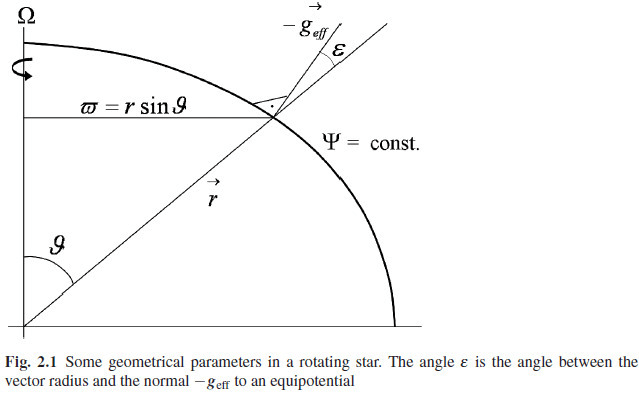
\includegraphics[width=(0.9\textwidth),height=(\textheight-11mm),keepaspectratio]{rotequi}
\caption{Geometrical parameters in rotating star.}
\end{figure}

Considerando la rotazione costante, cio\'e come corpo rigido, l'equazione del moto diventa
\begin{align*}
&\frac{1}{\rho}\nabla P=-\nabla\phi+\frac{1}{2}\Omega^2\nabla(r\sin{\theta})^2\\
&\vec{g}=-\nabla\phi=-\frac{Gm(r)}{r^2}\frac{\vec{r}}{r}
\end{align*}

Introduco un potenziale di rotazione
\begin{equation*}
-\nabla V=\Omega^2(r\sin{\theta})\Rightarrow V=-\frac{1}{2}\Omega^2(r\sin{\theta})^2
\end{equation*}

quindi l'equazione di Poisson diventa

\begin{align*}
&\nabla^2\Psi=4\pi G\rho-2\Omega\\
&\Psi=\phi+V
\end{align*}

e (barotropic stars) l'equazione di equilibrio idrostatico
\begin{equation*}
\frac{1}{\rho}\nabla P=-\nabla\Psi=g_{eff}
\end{equation*}

La forza centrifuga al polo \'e nulla quindi la superficie \'e un equipotenziale di $\frac{GM}{R_p}$, $R(\theta)$ \'e determinato da
\begin{equation*}
\frac{GM}{R(\theta)}+\frac{1}{2}\Omega^2R^2\sin^2{\theta}=\frac{GM}{R_p}
\end{equation*}

\clearpage

\subsection{Fluido in rotazione}

\begin{definition}{Parametro di deformazione}
Rapporto tra l'accelerazione centrifuga e l'accelerazione di gravit\'a: $u$.

\end{definition}

Definisco come parametro per descrivere la deformazione di un fluido autogravitante in rotaziane il rapporto tra l'attrazione gravitazionale e la forza centrifuga all'equatore
\begin{align*}
&u=\frac{\omega^2R^3}{GM}&\intertext{In termini di energia rotazionale e gravitazionale}\\
&E_{Rot}=\frac{1}{5}MR^2\omega^2\\
&E_{Gra}=\frac{3}{5}\frac{GM^2}{R}&\intertext{quindi}\\
&\frac{E_{Rot}}{E_{Gra}}=\frac{1}{3}\frac{\omega^2R^3}{GM}=\frac{1}{3}u\\
&u=\frac{3}{4}\frac{\omega^2}{\pi G \rho}&\intertext{per un corpo omogeneo}
\end{align*}

\subsection{Forma di equilibrio: argomento di Newton.}

Ellissoide di rotazione con semi-assi maggiori $a$ e minore $b=a\sqrt{1-e^2}$, $e$ \'e l'eccentricit\'a.

\begin{figure}[!ht]
\centering
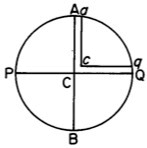
\includegraphics[width=(0.4\textwidth),height=(\textheight-11mm),keepaspectratio]{PEwell}
\caption{Colonne di fluido polare ed equatoriale.}
\end{figure}

Per densit\'a costante:
\begin{align*}
&ag_{eq}(1-u)=bg_{Pol}&\intertext{Primo membro: all'equatore l'accelerazione gravitazionale \'e diluita dall'accelerazione centrifuga (in corpo omogeneo sono proporzionali ad r). Il rapporto fra le due \'e uguale al valore sulla superficie.}\\
&ag_{eq}-a^2\omega^2=g_{Polo}a\sqrt{1-e^2}\\
&\epsilon=\frac{R_{eq}-R_{Polo}}{\exv{R}}=1-\sqrt{1-e^2}\approx\frac{e^2}{2}\\
&=1-\frac{b}{a}&\intertext{$\uparrow$ schiacciamento ai poli}\\
&\frac{g_{Polo}}{g_{eq}}=1+\frac{1}{5}\epsilon+O(\epsilon^2)&\intertext{quindi}\\
&(1-u)=(1-\epsilon)(1+\frac{1}{5}\epsilon)+O(\epsilon^2)\\
&=1-\frac{4}{5}\epsilon+O(\epsilon^2)&\intertext{da cui segue la relazione di Newton:}\\
&\epsilon=\frac{5}{4}u
\end{align*}

\clearpage

\subsection{MacLaurin spheroids}

Chiamo
\begin{align*}
&E_g=\frac{1}{2}\int\rho\Phi\,dV&\intertext{In caso di simmetria sferica: $\frac{d\Phi}{dr}=\frac{Gm(r)}{r^2}$}\\
&\chi=\frac{\omega^2}{2\pi G\rho}
\end{align*}

\begin{align*}
&e^2=\frac{a^2-b^2}{a^2}&\intertext{Along the series of increasing eccentricity $L$ and $E_g$ vary monotonically.}
\end{align*}

If we start with liquid selfgraviting body and feed in angular momentum $L$ also $\omega$ increases and e increses until $e\geq0.9299$ then $\omega$ decreses since moment of inertia increses faster than $\omega$. Before this, at $e=0.8127$, the McLaurin spheroid become unstable: the sequence of configuration shows a bifurcation and we have the Jacobi tri-axial ellipsoid (Jacobi ellipsoid of same mass and angular momentum has lower energi $E=E_g+E_{Rot}$)

\begin{figure}[!ht]
\centering
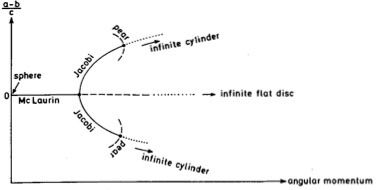
\includegraphics[width=(\textwidth),height=(\textheight-11mm),keepaspectratio]{McL2J}
\caption{Sequence of McLaurin and Jacobian equilibrium configurations of rotating incompressible fluid. a,b,c are 3 axis of an ellipsoid. Solid lines indicate dinamically or secularly stable configurations.}
\end{figure}

If there is a mechanism like friction which can transform macroscopic energy into heat spheroid become ellipsoid: the transition take place on the time-scale of friction.

\begin{figure}[!ht]
\centering
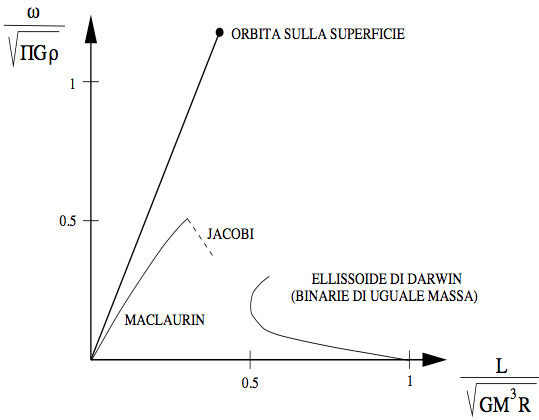
\includegraphics[width=(\textwidth),height=(\textheight-11mm),keepaspectratio]{Eq-shape}
\caption{Relazione $\omega-L$ per figure di equilibrio.}
\end{figure}

\clearpage


\chapter{Teorema del viriale: relazioni statistiche.}
\PartialToc

\section{Teorema del viriale}

\subsection{Thermal/kinetic energy}

\begin{align*}
&K=\int_0^R\overbrace{(+\frac{3}{2}\frac{K}{\mu m_u}T)}^{v^2}\rho 4\pi r^2\,dr\\
&=\overline{+\frac{3}{2}\frac{K}{\mu m_u}T}M\approx\SI{5e48}{\erg}
\end{align*}

\subsection{Teorema del viriale: equilibrio idrostatico.}

\begin{align*}
&\frac{1}{2}\TtwoDy{t}{I}=2K+\Omega\\
&2K=\sum_im_iv_i^2=\sum_i\scap{p_i}{v_i}&\intertext{$\scap{p_i}{v_i}$ measure rate of momentum transfer hence must be related to Pressure}\\
&P=\frac{1}{3}\int_pn(\vec{p})\scap{p}{v}d^3p&\intertext{confrontando le ultime due equazioni si ha:}\\
&2K=3\int_VP\,dV=3\int_M\frac{P}{\rho}\,dm(r)
\end{align*}

Il teorema del viriale si riscrive
\begin{align*}
&\frac{1}{2}\TtwoDy{t}{I}=\int_M\frac{3P}{\rho}\,dm(r)+\Omega&\intertext{Per equilibrio idrostatico}\\
&\frac{1}{2}\TtwoDy{t}{I}=0
\end{align*}

\subsection{$\gamma$-law equation of state.}

Se vale una relazione del tipo \mblock{P=(\gamma-1)\rho u} (per i gas ideali monoatomici con \mblock{\gamma=\frac{5}{3}}, \mblock{P=\frac{2}{3}\rho u})
\begin{equation*}
2K=3(\gamma-1)\int u\,dm
\end{equation*}

$K=E_i$ solo per $\gamma=\frac{5}{3}$: l'energia cinetica \'e uguale all'energia interna totale solo in determinate circostanze.

Il teorema del viriale si riscrive
\begin{equation*}
3(\gamma-1)E_i+\Omega=0
\end{equation*}

e scrivendo l'energia totale $W=E_i+\Omega$ ottengo la relazione esplicita tra energia totale ed energia potenziale gravitazionale per stelle idrostatiche in cui vale la relazione \mblock{P=(\gamma-1)\rho u}
\begin{equation*}
W=\frac{3\gamma-4}{3(\gamma-1)}\Omega
\end{equation*}



\subsection{Gravitational energy.}

Prendo un elemento di massa unitaria a distanza r: la sua energia potenziale dovuta alla massa entro r \'e $-\frac{Gm}{r}$. Quindi l'energia potenziale sommata su tutti gli elementi di massa $dm$ della stella \'e
\begin{equation*}
E_g=-\int_0^M\frac{Gm}{r}\,dm
\end{equation*}

L'energia $-E_g(>0)$ \'e l'energia necessaria ad espandere tutti gli strati a infinito: \'e l'energia liberata quando la stella si forma per contrazione di una gas rarefatto.



\subsection{Internal energy for ideal gas}

Per un gas ideale
\begin{align*}
&\frac{P}{\rho}=\frac{R}{\mu}T=(c_P-c_v)T=(\gamma-1)c_vT=\frac{2}{3}u&\intertext{$\uparrow$ ho usato: $\frac{R}{\mu}=c_P-c_v$. Per un gas monoatomico: $\gamma=\frac{c_P}{c_v}=\frac{5}{3}$ e $u=c_vT$ \'e l'energia interna del gas per unit\'a di massa}
\end{align*}


\subsection{Kinetic energy of the gas.}

\begin{align*}
&dE_k=\frac{3}{2}KT\,dN=\frac{3}{2}RT\,dm\\
&=\frac{3}{2}(c_P-c_V)T\,dm&\intertext{$dN$ \'e il numero di molecole nell'elemento di massa.}\\
&dU=c_VT\,dm&\intertext{quindi ricavo una relazione tra energia cinetica totale delle particelle di gas per unit\'a di massa ed energia interna per unit\'a di massa:}\\
&E_i=\frac{3}{2}(\gamma-1)U
\end{align*}


\subsection{Virial theorem for ideal monoatomic gas in hydrostatic equilibrium}

Il teorema del viriale connette due serbatoi di energia stellare.

\begin{align*}
&\int_0^M\frac{Gm}{r}\,dm=3\int_0^M\frac{P}{\rho}\,dm&\intertext{Il lato sinistro dell'equazione \'e $-E_g$: se la stella si espande/contrae $-E_g$ diminuisce/aumenta (valida per tempi grandi rispetto a $t_{hyd}$). $\uparrow$ deriva dalla seconda equazione fondamentale in forma Lagrangiana moltiplicata per $4\pi r^3$ integrata tra 0 ed M e la relazione $\downarrow$}\\
&\int_0^M4\pi r^3\frac{\partial P}{\partial m}\,dm\\
&=[4\pi r^3P]_0^M-\int_0^M12\pi r^2\frac{\partial r}{\partial m}P\, dm&\intertext{$\uparrow$ ho usato P(M)=0. Seconda equazione F. (equilibrio idrostatico): $\downarrow$}\\
&\frac{\partial P}{\partial m}=-\frac{Gm}{4\pi r^4}\\
&\frac{P}{\rho}=\frac{2}{3}u&\intertext{con $E_i=\int_0^Mu\,dm$:}\\
&E_g=-2E_i
\end{align*}


\subsection{Stima temperatura media.}

Star of uniform temperature and density composed of monoatomic ideal gas. The internal energy density is
\begin{align*}
&U=\frac{3}{2}nkT=\frac{3}{2}\rho\frac{N_AkT}{\mu}\si{\erg\per\cubic\cm}&\intertext{$\mu$ is the mean molecular weight per ion or atom}\\
&P=nkT=\frac{\rho N_AkT}{\mu}\\
&E_i=VU=\frac{3}{2}\frac{MN_AkT}{\mu}&\intertext{il teorema del viriale in questo caso ci dice che $E_i=-\frac{\Omega}{2}$, ($\gamma=\frac{5}{3}$)}\\
&\Omega=-\frac{3}{5}\frac{GM^2}{R}\\
&T=\num{4.09e6}\mu(\frac{M}{\msun{}})\expy{\frac{2}{3}}\rho\expy{\frac{1}{3}}\si{\kelvin}
\end{align*}



\subsection{Teorema del viriale per equazione di stato generale.}

Definisco parametro $\zeta$

\begin{align*}
&\zeta u=3\frac{P}{\rho}&\intertext{Gas ideale:}\\ &\zeta=3(\gamma-1)\xrightarrow{\gamma=\frac{5}{3}}2&\intertext{Pure photon gas:}\\
&P=\frac{1}{3}aT^4, u\rho=aT^4, \zeta=1
\end{align*}

Se $\zeta$ \'e costante nella stella ho una forma pi\'u generale del teorema del viriale
\begin{equation*}
\zeta E_i+E_g=0
\end{equation*}

\subsection{Coupling between $E_i$, $E_g$ and total energy.}

A change in total energy of the configuration is connected with change of its internal energy and with expansion or shrinking:
\begin{equation*}
W=E_i+E_g=(1-\zeta)E_i=\frac{\zeta-1}{\zeta}E_g
\end{equation*}

A gas of finite temperature must radiate
\begin{align*}
&L+\frac{dW}{dt}=0\\
&L=(\zeta-1)\frac{dE_i}{dt}=-\frac{\zeta-1}{\zeta}\frac{dE_g}{dt}
\end{align*}

Ho visto che $\dot{E_g}<0$ per contrazioni di tutti gli strati sferici e per un gas ideale l'equazione precedente da 
\begin{align*}
&L=-\frac{1}{2}\dot{E_g}=\dot{E_i}&\intertext{cio\'e met\'a dell'energia liberata dalla contrazione \'e irradiata nell'universo l'altra met\'a usata per scaldare la stella ($L>0,\dot{E_i}>0$)}
\end{align*}

Stars have negative specific heat: si scaldano mentre perdono energia.

\section{Kelvin-Helmholtz time-scale}

Definisco il tempo caratteristico per l'evoluzione di una stella in collasso: 
\begin{align*}
&L\approx|\frac{dE_g}{dt}|\\
&\tau_{KH}=\frac{E_i}{L}\propto\frac{|E_g|}{L}&\intertext{approssimando rozzamente $E_g$:}\\
&|E_g|\approx\frac{G\overline{m}^2}{\overline{r}}\approx\frac{GM^2}{2R}\\
&t_{KH}\approx\frac{GM^2}{2RL}
\end{align*}
\index{Kelvin-Helmholtz time-scale.}

For the sun $L=3.827 *10^{33}erg/s$ so $t_{KH}\approx1.6*10^7\,yr$.

There are phases in a stellar life when $E_g$ is the main energy source then the star evolves on Kelvin-Helmholtz time-scale.

In any case
\begin{align*}
&\TDy{m}{T}=-\frac{T}{P}\frac{Gm(r)}{4\pi r^4}\nabla\\
&\nabla=\TDly{P}{T}
\end{align*}

\chapter{Energy conservation and energy flux.}
\PartialToc

\section{Third basic equation of stellar structure}

\subsection{Prima legge della termodinamica. Conservazione energia interna.}

If stresses reduce to pure pressure \mblock{P_{ij}=P\delta_{ij}}
\begin{equation*}
\TDy{t}{q}=\TDy{t}{E}+P\TDof{t}(\frac{1}{\rho})=\TDy{t}{E}+P\TDof{t}V
\end{equation*}

equivalent form under asumption 1) $P(\rho,T)$, 2) $E(\rho,T)$, 3) No composition change due to nuclear reaction.

La prima legge della termodinamica esprime la conservazione dell'energia interna (per unit\'a di volume).

Le equazioni equivalenti utilizzando gli esponenti adiabatici $\Gamma_i$

\begin{align*}
&\Gamma_1=\Dcvar{\TDly{\rho}{P}}{Ad},\ \Gamma_3-1=\Dcvar{\TDly{\rho}{T}}{Ad},\\ &\frac{\Gamma_2-1}{\Gamma_2}=\Dcvar{\TDly{P}{T}}{Ad}
\end{align*}

\begin{align*}
&\TDy{t}{\ln{T}}=\frac{\Gamma_2-1}{\Gamma_2}\TDy{t}{\ln{P}}+\frac{\TDy{t}{q}}{c_PT}\\
&\TDy{t}{\ln{P}}=\Gamma_1\TDy{t}{\ln{\rho}}+\frac{\rho(\Gamma_3-1)}{P}\TDy{t}{q}
\end{align*}

Per un gas perfetto $\gamma=\frac{c_P}{c_v}=\Gamma_i$.


\subsection{Flusso di energia locale}
Chiamo $l(r)$ il flusso di energia totale verso l'esterno da una sfera di raggio $r$: energia per sec.

In $l(r)$ sono compresi il trasporto di energia attraverso radiazione, conduzione, convezione: are included only those fluxes that require a temperature gradient.

\begin{figure}[!ht]
\centering
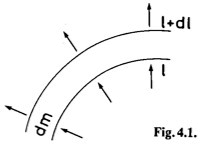
\includegraphics[width=(0.5\textwidth),height=\textheight,keepaspectratio]{localEF}
\caption{Contributo $dl$ da parte dello strato $dm$ fra $r$ e $r+\,dr$.}
\end{figure}

\subsection{Stationary case: only nuclear reaction contributes to $dl$.}

\begin{align*}
&dq=(\epsilon-\PDy{m}{l})\,dt&\intertext{Stato stazionario: il flusso di energia non modifica lo stato termodinamico del gas}\\
&dl=4\pi r^2\rho\epsilon\,dr=\epsilon\,dm\\
&\PDy{m}{l}=\epsilon
\end{align*}

\subsection{Non stationary case: also internal energy and exchange of work contribute to $dl$.}

\begin{align*}
&dq=(\epsilon-\PDy{m}{l})\,dt&\intertext{$\uparrow$ heat added per unit mass to the shell in the interval $dt$. Dalla prima legge della termodinamica ($dq=\,du+P\,dV$) ho:}\\
&\epsilon-\PDy{t}{u}-P\PDy{t}{v}=\epsilon-\PDy{t}{u}+\frac{P}{\rho^2}\PDy{t}{\rho}=\PDy{m}{l}&\intertext{In termini di $T$ e $P$ ho:}\\
&dq=c_P\,dT-\frac{\delta}{\rho}\,dP,\\
&(\delta=-\Dcvar{\PDly{T}{\rho}}{P}=\frac{T}{v}\Dcvar{\PDy{T}{v}}{P})&\intertext{ e quindi:}\\
&\PDy{m}{l}=\epsilon-c_P\PDy{t}{T}+\frac{\delta}{\rho}\PDy{t}{P}&\intertext{$\uparrow$ third basic equation of stellar structure.}
\end{align*}



\subsection{Considero la variazione di stato del gas: contributo alla luminosit\'a negativo/positivo.}

Definisco una funzione che contiene il contributo alla variazione di $l(r)$ per unit\'a di massa dovuta alla variazione dello stato termodinamico del gas

\begin{align*}
&\epsilon_{gas}=-\TDy{t}{q}=-T\PDy{t}{s}=-c_P\PDy{t}{T}+\frac{\delta}{\rho}\PDy{t}{P}\\
&=-c_PT(\frac{1}{T}\PDy{t}{T}-\frac{\nad}{P}\PDy{t}{P})\\
&\delta=-\Dcvar{\PDly{T}{\rho}}{P}=\frac{T}{v}\Dcvar{\PDy{T}{v}}{P}\\
&\nad{}=\Dcvar{\PDly{P}{T}}{s}=\frac{P\delta}{T\rho c_P}
\end{align*}

Surface luminosity of an expanding star can be smaller than energy produced in central core by nuclear reaction ($\epsilon>0$) since part of it is used to expand the star ($\epsilon_g<0$).

\subsection{Complete local energy equation}
La terza equazione fondamentale della struttura stellare \'e
\begin{align*}
&\PDy{m}{l}=\epsilon-c_P\PDy{t}{T}+\frac{\delta}{\rho}\PDy{t}{P}\\
&=\epsilon-\epsilon_{\nu}+\epsilon_g\\
&L_{\nu}=\int_0^M\epsilon_{\nu}\,dm&\intertext{$\uparrow$ neutrino luminosity. Condizioni al contorno:}\\
&l(0)=0\\
&l(R)=L
\end{align*}

\subsection{Energy conservation: total energy.}

Energia totale di una stella
\begin{align*}
&W=E_{Macro}+E_g+E_i+E_n&\intertext{$E_{Macro}$ is the kinetic energy of radial motion, $E_n$ is the nuclear energy content of the whole star. Energy balance:}\\
&\TDof{t}(E_{Macro}+E_g+E_i+E_n)+L+L_{\nu}=0&\intertext{Ottengo la stessa equazion $\uparrow$ integrando l'equazione locale rispetto a $dm$:}\\
&\int_0^M\,dm(\PDy{m}{l})=\int_0^M\,dm(\epsilon-\epsilon_{\nu}+\epsilon_{gas})\\
&\int\PDy{m}{l}=L,\quad\int-\epsilon_{\nu}\,dm=-L_{\nu},\\
&\int\epsilon\,dm=-\dot{E_n}&\intertext{Considero l'integrale di $\epsilon_{gas}$:}\\
&\int\,dm[-\PDy{t}{u}+\frac{P}{\rho^2}\PDy{t}{\rho}]=-\TDy{t}{E_i}-\TDy{t}{E_g}&\intertext{Il primo termine nelle parentesi quadre da}\\
&\int\,dm(-\PDy{t}{u})=-\TDy{t}{E_i}&\intertext{Per riconoscere il secondo derivo rispetto al tempo $E_g$ e uso il teorema del viriale \mblock{E_g=-2E_i=-\int\,dm3\frac{P}{\rho}}:}\\
&\dot{E_g}=-3\int_0^M\frac{\dot{P}}{\rho}\,dm+3\int_0^M\frac{P}{\rho^2}\dot{\rho}\,dm&\intertext{(Ricordo che:)}\\
&(-E_g=\int_0^M\frac{Gm}{r}\,dm=3\int_0^M\frac{P}{\rho}\,dm)&\intertext{Dalla condizione di equilibrio idrostatico ($E_{Macro}=0$) ricavo:}\\
&-3\int_0^M\frac{\dot{P}}{\rho}\,dm=\int_0^M4\pi r^3\PDy{m}{\dot{P}}\,dm\\
&=4\int_0^M\frac{Gm}{r}\frac{\dot{r}}{r}\,dm=4\dot{E_g}
\end{align*}

Per recuperare il termine $E_{Macro}$ devo usare l'equazione del moto
\begin{equation*}
\frac{1}{4\pi r^2}\PtwoDy{t}{r}=-\PDy{m}{P}-\frac{Gm}{4\pi r^4}
\end{equation*}
invece dell'equazione dell'equilibrio idrostatico.




\section{Time-scale consideration: sequenza principale, stelle pulsanti}

\subsection{Nuclear time-scale}

I consider a star balancing its energy loss by release of nuclear energy.

\begin{align*}
&\tau_n=\frac{E_n}{L}&\intertext{$E_n$ is the energy reservoir from which nuclear energy can be released. Hydrogen burning release:}\\
&Q=6.8*\sci{18}\,erg\,g^{-1}&\intertext{for a sun of only hydrogen}\\
&E_n=Q\msun=1.25*\sci{52}\,erg,\\
&\lsun=4*\sci{33}\,erg/\,sec\\
&\tau_n=3*\sci{18}s=\sci{11}\,yr
\end{align*}

\subsection{Ordine di grandezza termini energy equation}

Condizione $\tau_n\gg\tau_{KH}\gg\tau_{Hyd}$.

\begin{align*}
&|\PDy{m}{l}|\approx\frac{L}{M}\approx\frac{E_i}{\tau_{KH}M}\\
&\epsilon\approx\frac{L}{M}\approx\frac{E_n}{M\tau_n}\approx\frac{E_i}{\tau_{KH}M}&\intertext{$\uparrow$: $L$ \'e la stessa sia che la fonte di energia sia nucleare sia che sia l'energia potenziale gravitazionale. Introduco un tempo che caratterizza una determinata fase evolutiva della stella:}\\
&|c_P\PDy{t}{T}|\approx\frac{c_PT}{\tau}\approx\frac{E_i}{\tau M}\\
&|\frac{\delta}{\rho}\PDy{t}{P}|\approx\frac{c_PT}{\tau}\approx\frac{E_i}{\tau M}&\intertext{$\uparrow$ ho usato:}\\
&P=\frac{\rho}{\mu}RT,\ \delta=\frac{T}{v}\Dcvar{\PDy{T}{v}}{P},\\
&c_P=\Dcvar{\PDy{T}{q}}{P}=\Dcvar{\PDy{T}{u}}{P}+P\Dcvar{\PDy{T}{v}}{P}
\end{align*}

\subsection{Stelle di sequenza}

Nel caso $\tau\gg\tkh$ posso trascurare le derivate rispetto al tempo $(|\epsilon_g|\ll\epsilon)$, the energy equation becomes
\begin{align*}
\PDy{m}{l}=\epsilon&\intertext{This happens,ie, if H and He consumption sturns the evolution: $\tau=\tau_n$ and we have mechanical and thermal equilibrium}
\end{align*}

\subsection{Stelle pulsanti}

Nel caso $\tau\ll\tkh$ 
\begin{align*}
&|c_P\PDy{t}{T}|\approx|\frac{\delta}{\rho}\PDy{t}{P}|&\intertext{e cancellarsi a vicenda visto che $\TDy{t}{q}\approx0$ (change nearly adiabatic): a relatively small deviation from strictly adiabatic change can still be of order $\epsilon$. $\epsilon_g$ cannot be neglected.}
\end{align*}

For a pulsationg stars with \mblock{\tau=\thydro\ll\tkh} the variable luminosity is not due to changes of $\epsilon$ but $\epsilon_g$.

\end{document}